%*****************************************
\chapter{Formulas}\label{ch03:formulas}
%*****************************************

Excel workbooks are designed to allow you to create useful and complex calculations. In addition to doing arithmetic, you can use Excel to look up data, and to display results based on logical conditions. We will also look at ways to highlight specific results. These skills will be demonstrated in the context of a typical gradebook spreadsheet that contains the results for an imaginary Excel class.

\begin{center}
	\begin{objbox}{Learning Objectives}
		\begin{itemize}
			\setlength{\itemsep}{0pt}
			\setlength{\parskip}{0pt}
			\setlength{\parsep}{0pt}

			\item Use the Quick Analysis Tool to find the Total Points for all students and Points Possible.
			\item Write a division formula to find the Percentage for each student, using an absolute reference to the Total Points Possible.
			\item Write an IF Function to determine Pass/Fail where passing is $ 70\% $ or higher.
			\item Write a VLOOKUP to determine the Letter Grade using the Letter Grades scale.
			\item Use the TODAY function to insert the current date.
			\item Review common Error Messages using Smart Lookup to get definitions of some of the terms in your spreadsheet.
			\item Apply Data Bars to the Total Points values.
			\item Apply Conditional Formatting to the Percentage, Pass/Fail, and Letter Grade columns.
			\item Printing Review – Change to Landscape, Scale to Fit Columns on One Page and Set Print Area.
			
		\end{itemize}
	\end{objbox}
\end{center}

Figure \ref{03:fig01} shows the completed workbook that will be demonstrated in this chapter. Notice the techniques used in columns O and R that highlight the results of your calculations. Notice, also that there are more numbers on this version of the file than you will see in your original data file. These are all completed using Excel calculations.

\begin{figure}[H]
	\centering
	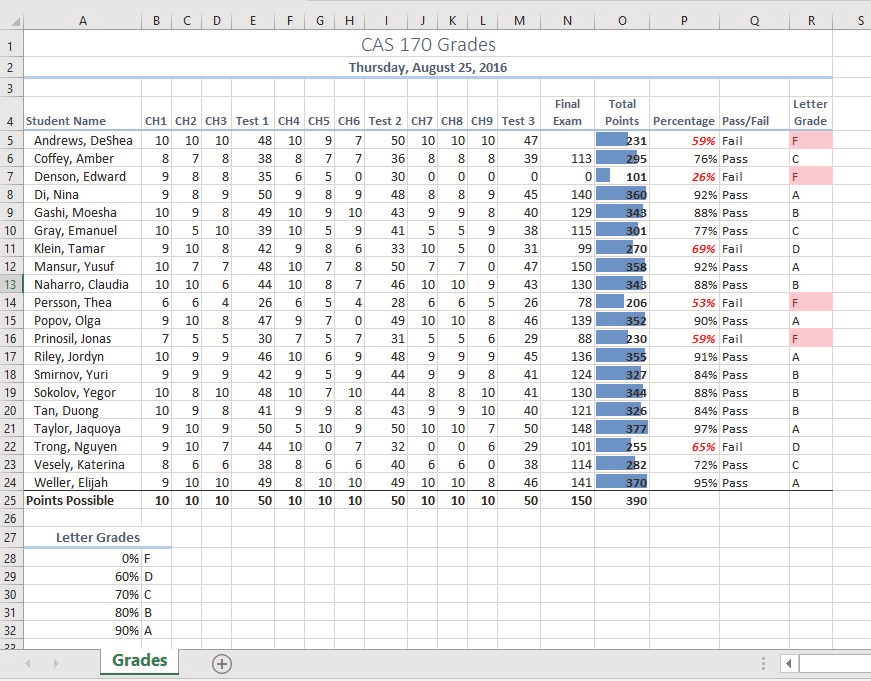
\includegraphics[width=\maxwidth{.95\linewidth}]{gfx/ch03_fig01}
	\caption{Completed Gradebook Worksheet}
	\label{03:fig01}
\end{figure}

\section{More on Formulas and Functions}

\begin{center}
	\begin{objbox}{Learning Objectives}
		\begin{itemize}
			\setlength{\itemsep}{0pt}
			\setlength{\parskip}{0pt}
			\setlength{\parsep}{0pt}
			
			\item Review the use of the \formatfunc{=MAX} function.
			\item Examine the Quick Analysis Tool to create standard calculations, formatting, and charts very quickly.
			\item Create Percentage calculation.

			\begin{itemize}
				\setlength{\itemsep}{0pt}
				\setlength{\parskip}{0pt}
				\setlength{\parsep}{0pt}

				\item Use the Smart Lookup tool to acquire additional information about percentage calculations.
				\item Review the use of Absolute cell reference in a division formula.
			\end{itemize}

		\end{itemize}
	\end{objbox}
\end{center}

\subsection{Another Use for =MAX}

Before we move on to the more interesting calculations we will be discussing in this chapter, we need to determine how many points it is possible for each student to earn for each of the assignments. This information will go into Row 25. The \formatfunc{=MAX} function is our tool of choice.

\textit{Data File: CH3 Data}

\begin{enumerate}
	\item Open the data file \textbf{CH3 Data} and save the file to your computer as \textbf{CH3 Gradebook}.
	\item Make \textsf{B25} the active cell.
	\item Start typing \formatfunc{=MAX} (See Figure \ref{03:fig02}). Note the explanation you see on the offered list of functions. You can either keep typing '(' or double click \textit{MAX} from the list.
\end{enumerate}

\begin{figure}[H]
	\centering
	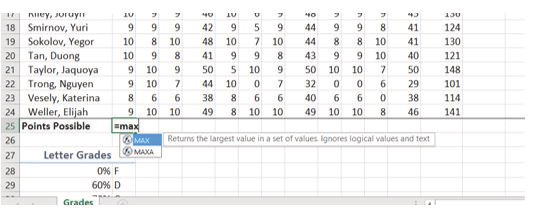
\includegraphics[width=\maxwidth{.95\linewidth}]{gfx/ch03_fig02}
	\caption{Entering a function}
	\label{03:fig02}
\end{figure}

\begin{enumerate}[resume]
	\item Select the range of numbers above row 25. Your calculation will be: \formatfunc{=MAX(B5:B24)}
	\item Now, use the Fill Handle to copy the calculation from Column B through Column N. Note that as you copy the calculation from one column to the next, the cell references change. The calculation in column B reads: \formatfunc{=MAX(B5:B24)}. The one in column N reads \formatfunc{=MAX(N5:N24)}. These cell references are relative references.
\end{enumerate}

By default, the calculations that Excel copies change their cell references relative to the row or column they are copied to. That makes sense. Column N should not display an answer that uses the values in column L.

If you want to see all the calculations you have just created, press \keystroke{Ctrl} + \keystroke{$ \sim $} (See Figure \ref{03:fig03}) \keystroke{Ctrl} + \keystroke{$ \sim $} displays the calculations (formulas). Pressing \keystroke{Ctrl} + \keystroke{$ \sim $} a second time will display calculations in the default view --- as values.

\begin{figure}[H]
	\centering
	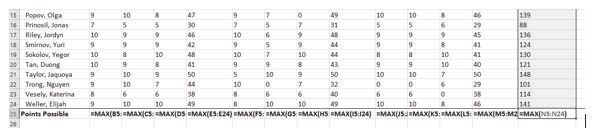
\includegraphics[width=\maxwidth{.95\linewidth}]{gfx/ch03_fig03}
	\caption{Relative References – Displayed as calculations.}
	\label{03:fig03}
\end{figure}

\subsection{Quick Analysis Tool}

The Quick Analysis Tool allows you to create standard calculations, formatting, and charts very quickly. In this exercise we will use it to insert the Total Points for each student in Column O.

Be sure to press \keystroke{Ctrl} + \keystroke{$ \sim $} to return your spreadsheet to the normal view (the formula results should display, not the formulas themselves).

\begin{enumerate}
	\item Select the range of cells \textsf{B5:N25}
	\item In the lower right corner of your selection, you will see the Quick Analysis tool (see Figure \ref{03:fig04}).
\end{enumerate}

\begin{figure}[H]
	\centering
	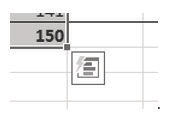
\includegraphics[width=\maxwidth{.95\linewidth}]{gfx/ch03_fig04}
	\caption{Quick Analysis Tool}
	\label{03:fig04}
\end{figure}

\begin{enumerate}[resume]
	\item When you click on it, you will see that there are a number of different options. This time we will be using the Totals option. In future exercises, we will use other options.
	\item Select Totals, and then the SUM option that highlights the right column (see Figure \ref{03:fig05}). Selecting that SUM option places \formatfunc{=SUM()} calculations in column O.
\end{enumerate}

\begin{figure}[H]
	\centering
	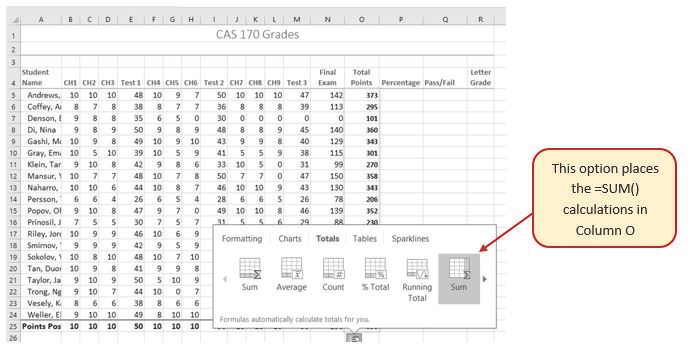
\includegraphics[width=\maxwidth{.95\linewidth}]{gfx/ch03_fig05}
	\caption{Quick Analysis Tool – Totals, Sum Column}
	\label{03:fig05}
\end{figure}

\subsection{Percentage Calculation}

Column P requires a Percentage calculation. Before we launch in to creating a calculation for this, it might be handy to know precisely what it is we are looking for. If you are connected to the internet and are using Excel 2016, you can use the Smart Lookup tool to get more information.

\begin{enumerate}
	\item Select cell \textsf{P4}.
	\item Find the \textbf{Smart Lookup} tool on the \textbf{Review} tab (see Figure \ref{03:fig06}).
	\item Press the \textbf{Smart Lookup} tool to find more about Percentage calculations. If this is the first time you have used the Smart Lookup tool, you may need to respond to a statement about your privacy. Press the \textbf{Got it} button.
\end{enumerate}

I think the first Wikipedia article does a pretty good job explaining the calculation, don't you?

\begin{figure}[H]
	\centering
	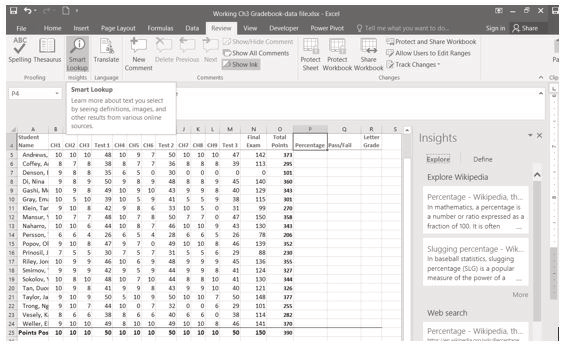
\includegraphics[width=\maxwidth{.95\linewidth}]{gfx/ch03_fig06}
	\caption{Smart Lookup tool}
	\label{03:fig06}
\end{figure}

Now that we know what is needed for the Percentage calculation, we can have Excel do the calculation for us. We need to divide the \textbf{Total Points} for each student by the \textbf{Total Points} of all the \textbf{Points Possible}. Notice that there is a different number on each row for each student. But, there is only one \textbf{Total Points Possible} --- the value that is in cell \textsf{O25}.

1. Make sure that P5 is your active cell.
2. Press = then select cell O5. Press /, then cell O25. Your calculation should look like this: =O5/O25. The result of the formula should be 0.95641026. (So far, so good. DeShea Andrews is doing well in this class – with a percentage grade of almost 96\%. Definitely an ``A''!)
3. Next use the Fill handle to copy the calculation down through row 24 to calculate the other students' grades. You should get the error message $ \#DIV/0! $. This error message reminds us that you cannot divide a number by $ 0 $ (zero). The calculation in \textsf{P9} reads $ =O9/O29 $. The first cell reference is correct --- it points to Moesha Gashi's total points for the class. But the second reference is wrong. It points to an empty cell, \textsf{O29}.

Before copying the calculation, we have to make the second reference (\textsf{O25}) an absolute cell reference. That way, when we copy the formula down, the cell reference for \textsf{O25} will be locked and will not change.

\begin{enumerate}
	\item Make \textsf{P5} the active cell. In the Formula Bar click on O25 (see Figure \ref{03:fig07}).
	\item Press \keystroke{F4} (on the function keys at the top of your keyboard). That will make the \textsf{O25} reference absolute. It will not change when you copy the calculation (see Figure \ref{03:fig08}). (If you are working on a laptop and do not have an \keystroke{F4} function key, you can type in a \$ before the \textsf{O} and another one before the \textsf{25}.)
	\item The calculation now looks like \formatfunc{=O5/\$O\$25}.
	\item Use the Fill Handle to copy the formula down through \textsf{P24} again. Now the formula has the correct values for all students.
\end{enumerate}

\begin{figure}[H]
	\centering
	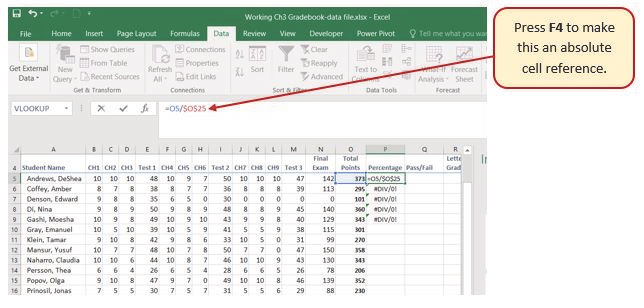
\includegraphics[width=\maxwidth{.95\linewidth}]{gfx/ch03_fig07}
	\caption{Editing a formula}
	\label{03:fig07}
\end{figure}

\begin{figure}[H]
	\centering
	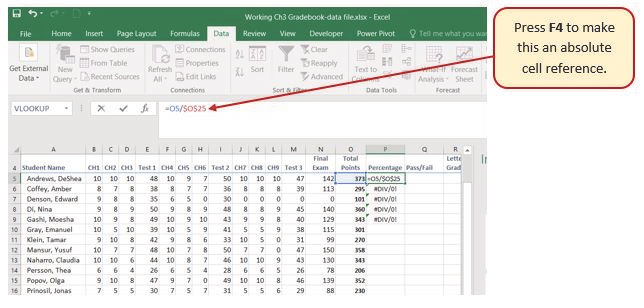
\includegraphics[width=\maxwidth{.95\linewidth}]{gfx/ch03_fig08}
	\caption{Absolute Cell reference – press F4}
	\label{03:fig08}
\end{figure}

Those long decimals are a bit nonstandard so they should be changed to a percent by applying cell formatting.

\begin{enumerate}
	\item Select the range \textsf{P5:P24}.
	\item On the Home tab, in the Number Group, select the \% (Percent Style) button.
\end{enumerate}

\begin{center}
	\begin{sklbox}{Skill Refresher}
		\textbf{Absolute References}
		\\
		\begin{itemize}
			\setlength{\itemsep}{0pt}
			\setlength{\parskip}{0pt}
			\setlength{\parsep}{0pt}

			\item Click in front of the column letter of a cell reference in a formula or function that you do not want altered when the formula or function is pasted into a new cell location.
			\item Press the \keystroke{F4} key or type a dollar sign (\$) in front of the column letter and row number of the cell reference.
						
		\end{itemize}
	\end{sklbox}
\end{center}

\begin{center}
	\begin{tkwbox}{Key Take-Aways}
		\textbf{Functions}
		\\
		\begin{itemize}
			\setlength{\itemsep}{0pt}
			\setlength{\parskip}{0pt}
			\setlength{\parsep}{0pt}

			\item Functions can be created using cell ranges or selected cell locations separated by commas. Make sure you use a cell range (two cell locations separated by a colon) when applying a statistical function to a contiguous range of cells.
			\item To prevent Excel from changing the cell references in a formula or function when they are pasted to a new cell location, you must use an absolute reference. You can do this by placing a dollar sign (\$) in front of the column letter and row number of a cell reference or by using the \keystroke{F4} function key.
			\item The $ \#DIV/0 $ error appears if you create a formula that attempts to divide a constant or the value in a cell reference by zero.
			
		\end{itemize}
	\end{tkwbox}
\end{center}

\section{Logical and Lookup Functions}

\begin{center}
	\begin{objbox}{Learning Objectives}
		\begin{itemize}
			\setlength{\itemsep}{0pt}
			\setlength{\parskip}{0pt}
			\setlength{\parsep}{0pt}

			\item Use an \formatfunc{IF} Function to make logical comparisons between a value and what you expect.
			\item Create a \formatfunc{VLOOKUP} calculation to look up information in a table.
			\item Understand error messages.
			\item Understand how to enter and format Date/Time Functions.
			
		\end{itemize}
	\end{objbox}
\end{center}

In addition to doing arithmetic, Excel can do other kinds of functions based on the data in your spreadsheet. In this section we will use an \formatfunc{=IF} function to determine whether a student is passing or failing the class. Then, we will use a \formatfunc{=VLOOKUP} function to determine what grade each student has earned.

\subsection{If Function}

The \formatfunc{IF} function is one of the most popular functions in Excel. It allows you to make logical comparisons between a value and what you expect. In its simplest form, the \formatfunc{IF} function says something like, ``If the value in a cell is what you expect (true) then do this; otherwise do that.

The \formatfunc{IF} function has three arguments.

\begin{itemize}
	\item \textbf{Logical test}. this is the test to see if the value in a selected cell is what was expected. A test can be something like ``$ B7=14 $'' or ``$ B7>12 $'' or ``$ B7<6 $.''
	\item \textbf{Value\_if\_true}. What to do if the requirements in the logical test are met, for example, if \textsf{B7} is equal to $ 14 $. For this argument you can type text like ``True,'' or ``On budget!'' Or you could insert a calculation, like $ B7*2 $. That is, if \textsf{B7} equals $ 14 $ then multiply it by $ 2 $. Or, if Excel should put nothing at all in the cell then type ``'' (two quotes).
	\item \textbf{Value\_if\_false}. What to do if the requirements in the logical test are \textit{NOT} met; for example, if \textsf{B7} does \textit{NOT} equal $ 14 $. To have Excel do nothing, then type empty double quotes. Of course, Excel can also enter whatever text or calculation is desired.
\end{itemize}

In column Q we would like Excel to tell us whether a student is passing or failing the class. Student who score $ 70\% $ or better will pass the class; but scores less than $ 70\% $ are failing.

\begin{enumerate}
	\item Make sure that \textsf{Q5} is the active cell.
	\item On the Formulas tab, in the Function Library, find the \formatfunc{IF} function on the Logical pulldown menu (see Figure \ref{03:fig09}).
\end{enumerate}

\begin{figure}[H]
	\centering
	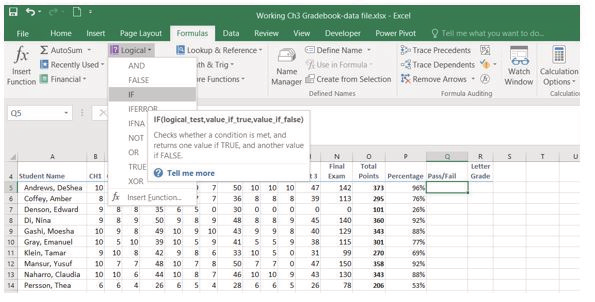
\includegraphics[width=\maxwidth{.95\linewidth}]{gfx/ch03_fig09}
	\caption{IF Function}
	\label{03:fig09}
\end{figure}

Now you will see the \formatfunc{IF} Function dialog box, with a place to enter each of the three arguments.

\begin{enumerate}
	\item Click in the box for \textbf{Logical Test}. To test whether a student's score is less than $ 0.7 $ enter \formatfunc{P5<0.7}.
	\item Click in the box for \textbf{Value\_if\_true}. If the student's score is less than $ 0.7 $, then they are failing the class. In this box, type \textbf{Fail}.
	\item Click in the box for \textbf{Value\_if\_false}. If the student's score is \textit{NOT} less than $ 0.7 $, then they are passing the class. In this box, type \textbf{Pass}.
	\item Make sure that the dialog box matches Figure \ref{03:fig10}.
\end{enumerate}

\begin{figure}[H]
	\centering
	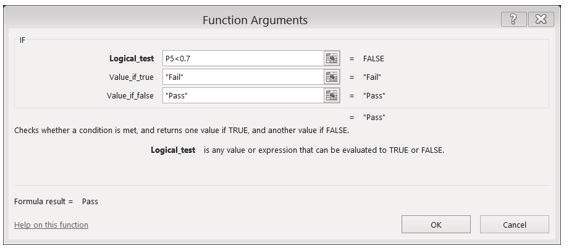
\includegraphics[width=\maxwidth{.95\linewidth}]{gfx/ch03_fig10}
	\caption{IF Function Dialog Box}
	\label{03:fig10}
\end{figure}

Notice that as each box is filled Excel offers a brief explanation of the contents (in the middle below the boxes.) In the lower left hand corner is the results of the calculation. In this case, DeShae is passing the class. Below that is a link to Help on this function. Selecting this link will open Excel help for this function, along with detailed information on how it works.

\begin{enumerate}[resume]
	\item Once the required arguments are entered and checked, press OK. The text ``Pass'' should be displayed in \textsf{Q5} because DeShae is passing the class.
	\item Use the Fill handle to copy the \formatfunc{IF} function down through row 24.
	\item Click on \textsf{Q5}. The formula bar should display the \formatfunc{IF} calculation: \formatfunc{=IF(P5<0.7,''Fail'',''Pass'')} (see Figure \ref{03:fig11}).
\end{enumerate}

\begin{figure}[H]
	\centering
	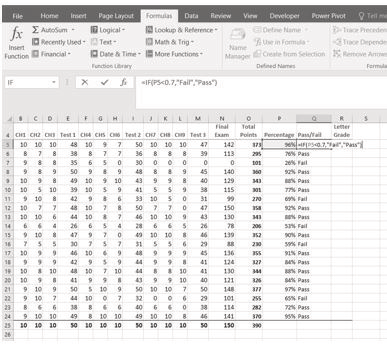
\includegraphics[width=\maxwidth{.95\linewidth}]{gfx/ch03_fig11}
	\caption{IF Function Results}
	\label{03:fig11}
\end{figure}

\subsection{Vlookup Function}

A \formatfunc{VLOOKUP} function is used to look up information in a table. Sometimes that table is on a different sheet in the workbook, though it can be in another file entirely. In this case, all students' grades are determined on their percentage score. The table that defines the scores and the grades is in \textsf{A28:B32}.

There are four pieces of information that needed to build the \formatfunc{VLOOKUP} syntax. 

\begin{itemize}
	\item The value to look up, also called the \textbf{Lookup\_value}. In lthe example, the lookup value will be the student's percentage score in column P.
	\item The \textbf{Table\_array} is the range (table) where the lookup values are located. In this example the table of percentages and corresponding letter grades is in the range \textsf{A28:B32}. The lookup value should always be in the first column in the table array for \formatfunc{VLOOKUP} to work correctly. 
	\item The \textbf{Col\_index\_num} is the column number in the range that contains the value to return. In this example, \textsf{A28:B32} is the Table\_array range so column A is the first column (1), column B is the second column (2), and so on if there were other columns. To return the grade in column B, the number 2 would be entered as the Col\_index\_num.
	\item The \textbf{Range\_lookup} is TRUE for an \textit{approximate} match or FALSE for an exact match. If this is left blank the default value will be TRUE, or an approximate match.
\end{itemize}

Follow these steps to create the \formatfunc{VLOOKUP} to display the correct Letter Grade in column R.

\begin{enumerate}
	\item Make sure that \textsf{R5} is the active cell.
	\item On the Formulas tab in the Function Library, find the \formatfunc{VLOOKUP} function on the Lookup \& Reference pull-down menu (see Figure \ref{03:fig12}).
\end{enumerate}

\begin{figure}[H]
	\centering
	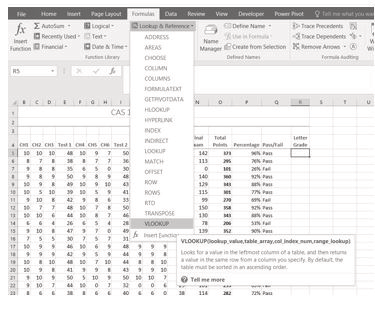
\includegraphics[width=\maxwidth{.95\linewidth}]{gfx/ch03_fig12}
	\caption{VLOOKUP Function}
	\label{03:fig12}
\end{figure}

Fill in the dialog box so that it looks like Figure \ref{03:fig13}.

\begin{itemize}
	\item \textbf{Lookup\_value}. Specify the percentage score, which is in cell \textsf{P5} for the first student.
	\item \textbf{Table\_array}. This is the range that contains the value to be returned by the function. In this case, that range is \textsf{A28:B32}. Note that this range does \textit{NOT} include the label in row 27; just the actual data. The cell references for the Table\_array need to be absolute: \textsf{\$A\$28:\$B\$32}. When this function is copied to other cells the cell references should not change.
	\item \textbf{Col\_index\_number}. This is the column in the table array range that includes the information that should be returned. In this case, the grades are in the 2nd column of the range so the column index will be $ 2 $.
	\item \textbf{Range\_lookup}. Since an approximate match is appropriate for this application the default value of TRUE is acceptable, so do not enter anything for this argument.
\end{itemize}

\begin{enumerate}[resume]
	\item Be sure to observe the helpful definitions that Excel offers while filling in the \formatfunc{VLOOKUP} dialog box.
	\item When the dialog box is complete, press OK.
	\item The calculation in the formula bar is: \formatfunc{=VLOOKUP(P5,\$A\$28:\$B\$32,2)}
	\item Use the fill handle to copy the function down through row $ 24 $. The results displayed should match Figure \ref{03:fig13}.
\end{enumerate}

\begin{figure}[H]
	\centering
	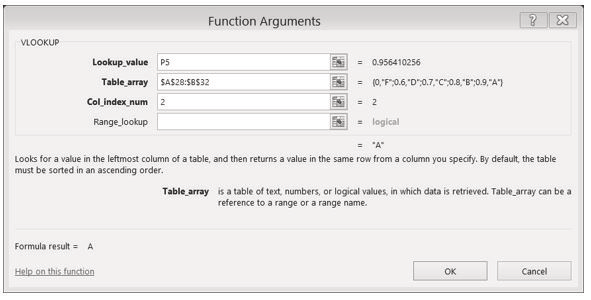
\includegraphics[width=\maxwidth{.95\linewidth}]{gfx/ch03_fig13}
	\caption{VLOOKUP completed dialog box}
	\label{03:fig13}
\end{figure}

\begin{figure}[H]
	\centering
	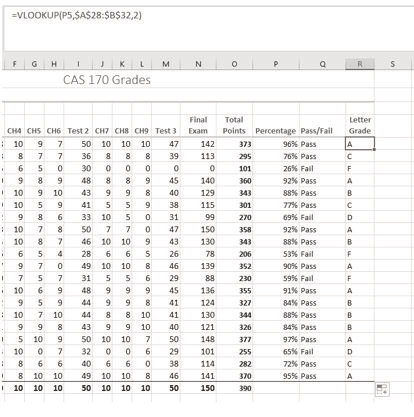
\includegraphics[width=\maxwidth{.95\linewidth}]{gfx/ch03_fig14}
	\caption{VLOOKUP Complete}
	\label{03:fig14}
\end{figure}

What if the \formatfunc{VLOOKUP} function does not work as expected? In this case, a mistake was made in either the calculation of the \% scores or there is an error in the \formatfunc{VLOOKUP} function. To make repairs to the function, make sure that \textsf{R5} is the active cell. On the Formula bar, press the Insert Function button (see Figure \ref{03:fig15}). That will reopen the dialog box to make repairs. A common error is to forget to make the cell references for the Table\_array absolute. Press OK when the correction is completed and then recopy the corrected function.

\begin{figure}[H]
	\centering
	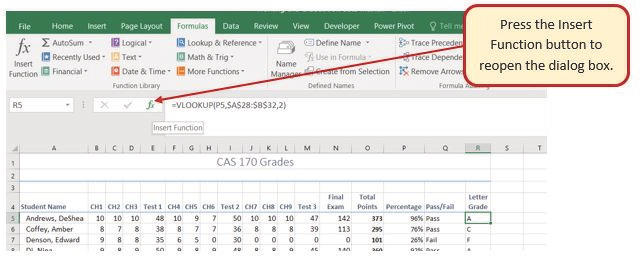
\includegraphics[width=\maxwidth{.95\linewidth}]{gfx/ch03_fig15}
	\caption{Insert Function}
	\label{03:fig15}
\end{figure}

\subsection{Error Messages}

Sometimes Excel notices errors in the calculations and may post a slightly mysterious error message. A list of common error messages can be found in Table \ref{03:tab01}.

{\small
	\begin{longtable}{p{0.75in}p{3.50in}} %Max width: 4.25in
		\textbf{Message} & \textbf{What Went Wrong} \endhead
		\hline \\
		$ \#DIV/0! $ & A number is being divided by a zero ($ 0 $) or by an empty cell.\\
		\#NAME & A cell range name in the formula is not defined. Frequently this error occurs because the name is entered incorrectly.\\
		\#N/A & The formula refers to an empty cell, so no data is available for computing the formula. Sometimes people enter \textit{N/A} in a cell as a placeholder to signal the fact that data is not entered yet. Revise the formula or enter a number or formula in the empty cells.\\
		\#NULL & The formula refers to a cell range that Excel cannot understand. Make sure that the range is entered correctly.\\
		\#NUM & An argument you use in your formula is invalid.\\
		\#REF & The cell or range of cells that the formula refers to are not there.\\
		\#VALUE & The formula includes a function that was used incorrectly, takes an invalid argument, or is misspelled. Make sure that the function uses the right argument and is spelled correctly.\\
		\caption{Common Error Messages}
		\label{03:tab01}
	\end{longtable}
}

\subsection{Date Functions}

Very often dates and times are an important part of Excel data. Numbers that are correct today may not be accurate tomorrow so it is frequently useful to include dates and times on your spreadsheets.

These dates and times fall into two categories, ones that:

\begin{itemize}
	\item \textbf{Remain the same.} For instance, if a spreadsheet includes data for May 15th then that date should not change each time the spreadsheet is accessed.
	\item \textbf{Change to reflect the current date/time.} When it is important to have the current date or time on a spreadsheet then Excel should update the information regularly.
\end{itemize}

Take a look at the list of Date and Time functions offered in the Function Library on the Formulas tab (see Figure \ref{03:fig16}).

\begin{figure}[H]
	\centering
	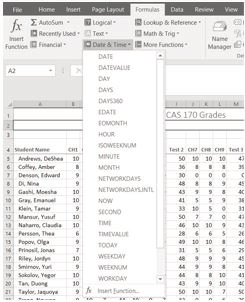
\includegraphics[width=\maxwidth{.95\linewidth}]{gfx/ch03_fig16}
	\caption{Date \& Time Functions}
	\label{03:fig16}
\end{figure}

For our gradebook, we want the date and time to be displayed in \textsf{A2}, and it needs to update whenever the workbook file is opened.

1. Make A2 your active cell. Notice that A2 extends all the way from column A to Column R.
Previously, someone has used the Merge \& Center tool on this cell to make it match the title
above.
2. On the Formulas tab, in the Function Library, select NOW from the Date \& Time drop-down
list and then click OK.
3. The result you will see in the formula bar is: =NOW(). The result you will see in A2 depends on
the current date and time.The NOW function is a very handy function. It takes no arguments

and is Volatile! That is not as alarming as it may seem. This just means that you don’t need to
give it any more information to do its job and that your results will change frequently.You can
update the date and time whenever you want – you don’t have to wait until you open the
workbook again.
4. Make sure that A1 is your active cell and press the F9 function key (along the top of your
keyboard.) The time will update.

Excel will update this field independently whenever you save and re-open the file, or print it. It may
happen more frequently than that – depending on how you have set this up in your installation of
Excel.

Another variation of the current date is the TODAY function. Let’s try that one next.

1. Make sure A2 is your active cell. Press Delete to remove the NOW function.
2. From the Date \& Time drop-down list in the Function Library on the Formulas tab (see Figure
3.16), select TODAY and then click OK.
3. The result you will see in the formula bar is: =TODAY(). The result you will see in A2 depends
on the current date.Since we haven’t asked for the time, the time you are seeing is likely 12:00.
That is not very helpful so we need to change the format of the date.
4. On the Home tab, in the Number group, press the Number Format Launch button (see Figure
3.17).
5. In the Format Cells dialog box, click the Number tab. Choose the Date category and select
Wednesday, March 14, 2012 (this format is called Long Date).
6. The current day and date will display in A2.


\begin{figure}[H]
	\centering
	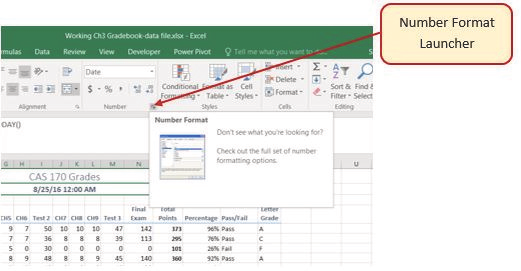
\includegraphics[width=\maxwidth{.95\linewidth}]{gfx/ch03_fig17}
	\caption{Number Format Launcher}
	\label{03:fig17}
\end{figure}





Keyboard Shortcuts


Sometimes you want the date or the time to show up in your spreadsheet, but you don’t want it to change. You can simply
type in the date or time. Or, you can use shortcut keys.

• CTRL; (semi colon) will bring you the current date

• CTRL: (colon or CTRL SHIFT ; ) will bring you the current time.


\begin{center}
	\begin{tkwbox}{Key Take-Aways}
		\textbf{Date Functions}
		\\
		\begin{itemize}
			\setlength{\itemsep}{0pt}
			\setlength{\parskip}{0pt}
			\setlength{\parsep}{0pt}

			\item Functions don’t always have to be about arithmetic. Excel provides functions that will help you perform logical evaluations, look things up, and work with dates and times.
			\item Excel displays error messages when your formulas and functions are not constructed properly.
			
		\end{itemize}
	\end{tkwbox}
\end{center}


\section{Conditional Formatting}

\begin{center}
	\begin{objbox}{Learning Objectives}
		\begin{itemize}
			\setlength{\itemsep}{0pt}
			\setlength{\parskip}{0pt}
			\setlength{\parsep}{0pt}

			\item Use Conditional Formatting techniques to provide flexible highlighting, applying specified formatting only
			when certain conditions are met. Techniques include:
			
			\item Data bars — to make it easy to visualize values in a range of cells.
			
			\item Cells Rules — to highlight values that match the requirements you specify.
			
		\end{itemize}
	\end{objbox}
\end{center}







You now have all the calculations you need in your CAS 170 Grades spreadsheet. There is a lot of
data here. To make it easier to pick out the most important pieces of data, Excel provides Conditional
Formatting. The best thing about Conditional Formatting is that it is flexible, applying specified
formatting only when certain conditions are met.

1. Select the values in the Total Points column (O5:O24).
2. At the bottom of your selection, click on the Quick Analysis Tool. On the Formatting tab, select
Data Bars (see Figure 3.18).

Excel places blue bars on top of your values; long blue bars for larger numbers, shorter ones for
smaller numbers. This makes it easier to see how well each student did in the class – without having
to look at the specific numbers.


\begin{figure}[H]
	\centering
	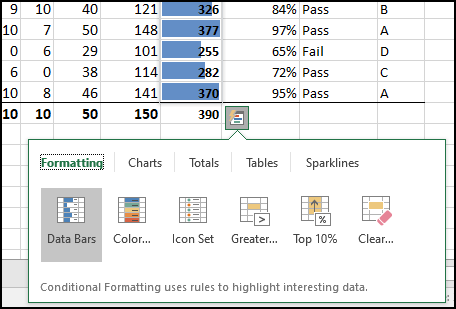
\includegraphics[width=\maxwidth{.95\linewidth}]{gfx/ch03_fig18}
	\caption{Data Bars on the Quick Analysis tool}
	\label{03:fig18}
\end{figure}


Another way to apply Data Bars is to:

• Select the range that needs data bars
• On the Home tab, in the Styles group, select Data Bars from the Conditional Formatting tool.
• From there you can select data bars of different colors and opacities (see Figure 3.19).


\begin{figure}[H]
	\centering
	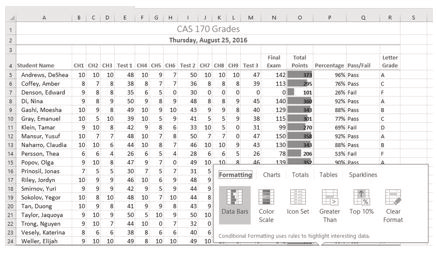
\includegraphics[width=\maxwidth{.95\linewidth}]{gfx/ch03_fig19}
	\caption{Data Bars on the Conditional Formatting tool}
	\label{03:fig19}
\end{figure}




It is even more important to highlight the students who are failing in the class. To practice further
with Conditional Formatting we will do that in two places, in the Percentages column and on the



Letter Grade column. To start with, we want any F letter grades to be formatted with a light red fill
color and dark red text.

1. Select the Letter Grades (R5:R24).
2. On the Home tab, in the Styles group, select Highlight Cell Rules from the Conditional
Formatting tool (see Figure 3.20).
3. Select Equal To
4. Fill out the Equal to dialog box so that cells that are equal to: F have Light Red Fill with Dark
Red Text (see Figure 3.21).



\begin{figure}[H]
	\centering
	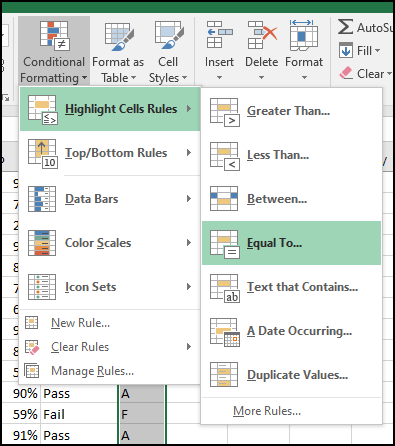
\includegraphics[width=\maxwidth{.95\linewidth}]{gfx/ch03_fig20}
	\caption{Conditional Formatting Equal To}
	\label{03:fig20}
\end{figure}


\begin{figure}[H]
	\centering
	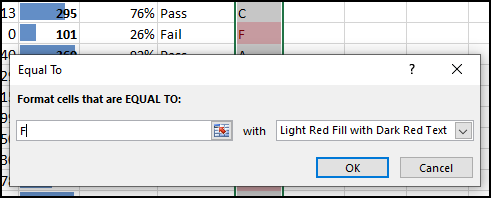
\includegraphics[width=\maxwidth{.95\linewidth}]{gfx/ch03_fig21}
	\caption{Conditional Formatting Equal To Dialog Box}
	\label{03:fig21}
\end{figure}




Let’s try that one more time – to highlight those students who are passing the class. This time we will
use the Pass/Fail text in the Pass/Fail column. If the text for a student is Pass we want the cell to be
formatted with a yellow fill with dark yellow text.

1. Select the Pass/Fail grades (Q5:Q24).
2. On the Home tab, in the Styles group, select Highlight Cell Rules from the Conditional
Formatting tool (see Figure 3.20).
3. Select Equal To
4. Fill out the Equal to dialog box so that cells that are equal to: Pass have Yellow Fill with Dark
Yellow Text. (To find the Yellow Fill with Dark Yellow text option, click the the down arrow at
the end of the last (with) box).

You do not have to use the default styles to make your data stand out. You can set any formatting
you want. When you do, it is probably a good idea to include other styling in addition to color. Your
spreadsheet might be printed in black and white. You would hate to lose your Conditional formatting.
Now we are going to use conditional formatting to display any Percentages that are less than 60%
with red text formatted in bold and italic.

1. Select the Percentage grades (P5:P24).
2. On the Home tab, in the Styles group, select Highlight Cell Rules from the Conditional
Formatting tool (see Figure 3.20).
3. Select Less Than
4. Fill out the Less Than dialog box so that cells that are less than .6 will be have conditional
formatting. But, instead of using the default red text on a light red fill, press the down arrow at
the end of that box and select Custom Format.

5. On the Font tab of the Format Cells dialog box, in the Font style box, select Bold Italic. In the
Color box, select Red (see Figure 3.22).
6. Press OK. Then press OK again.


\begin{figure}[H]
	\centering
	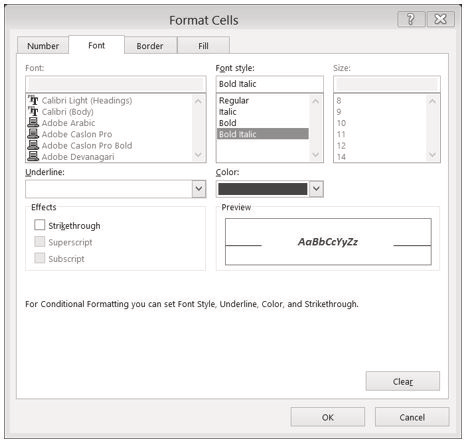
\includegraphics[width=\maxwidth{.95\linewidth}]{gfx/ch03_fig22}
	\caption{Conditional Formatting Custom Format Cells Dialog box}
	\label{03:fig22}
\end{figure}



Conditional Formatting is valuable in that it reflects the current data. It changes to reflect changes in
the data. To test this, delete DeShea’s final exam score. (Select N5. Press Delete on your keyboard.)
Suddenly, DeShae is failing the course and the Conditional Formatting reflects that. This is a little
unfair to DeShae – who has worked so hard this quarter. Let’s give him back his grade. Press CTRL Z
(Undo). His test score reappears and the Conditional formatting reflects that as well.

\subsection{Making Changes}

What if you have made a mistake with your Conditional Formatting? Or, you want to delete it
altogether? You can use the Conditional Formatting Manage Rules tool. In our example, we want
to remove the conditional formatting rule that formats the Pass text with yellow. We are also going
to modify the minimum passing percentage for the conditional formatting rule that is applied to the
percentages.

1. On the Home Tab, in the Styles Group, select Manage Rules at the very bottom of the
Conditional Formatting drop-down list.
2. Show formatting rules for: This Worksheet (see Figure 3.23).


3. We don’t really need to highlight the students who are passing the class, so select that rule in the
Rules Manager and press the Delete Rule button.


\begin{figure}[H]
	\centering
	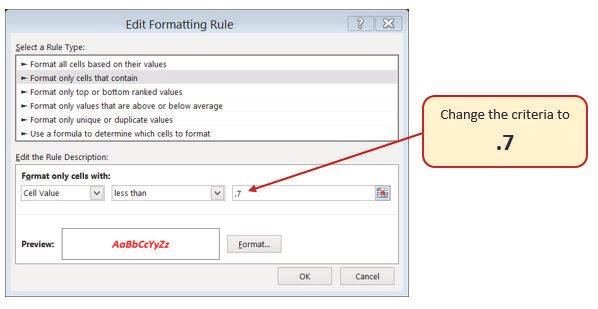
\includegraphics[width=\maxwidth{.95\linewidth}]{gfx/ch03_fig23}
	\caption{Conditional Formatting Manage Rules}
	\label{03:fig23}
\end{figure}



In a previous exercise (the IF function), we decided that students were failing if they got a
percentage score of less than 70\%, so the Conditional Formatting rule in the Percentage column
needs repair.
4. Select the rule that reads Cell Value <0.6.
5. Select the Edit Rule button, and change the .6 to .7 (see Figure 3.24).
6. Click OK (or Apply) twice. Double check that your completed workbook matches Figure 3.25.


\begin{figure}[H]
	\centering
	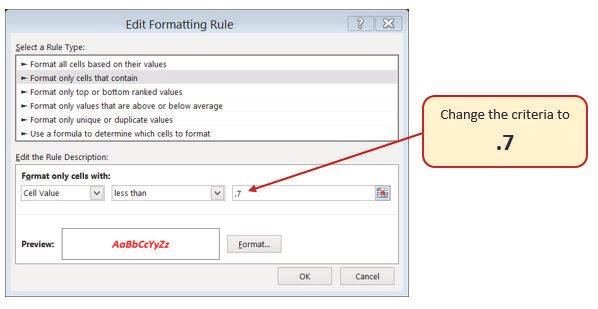
\includegraphics[width=\maxwidth{.95\linewidth}]{gfx/ch03_fig24}
	\caption{Conditional Formatting Edit Formatting Rule Dialog box}
	\label{03:fig24}
\end{figure}

\begin{figure}[H]
	\centering
	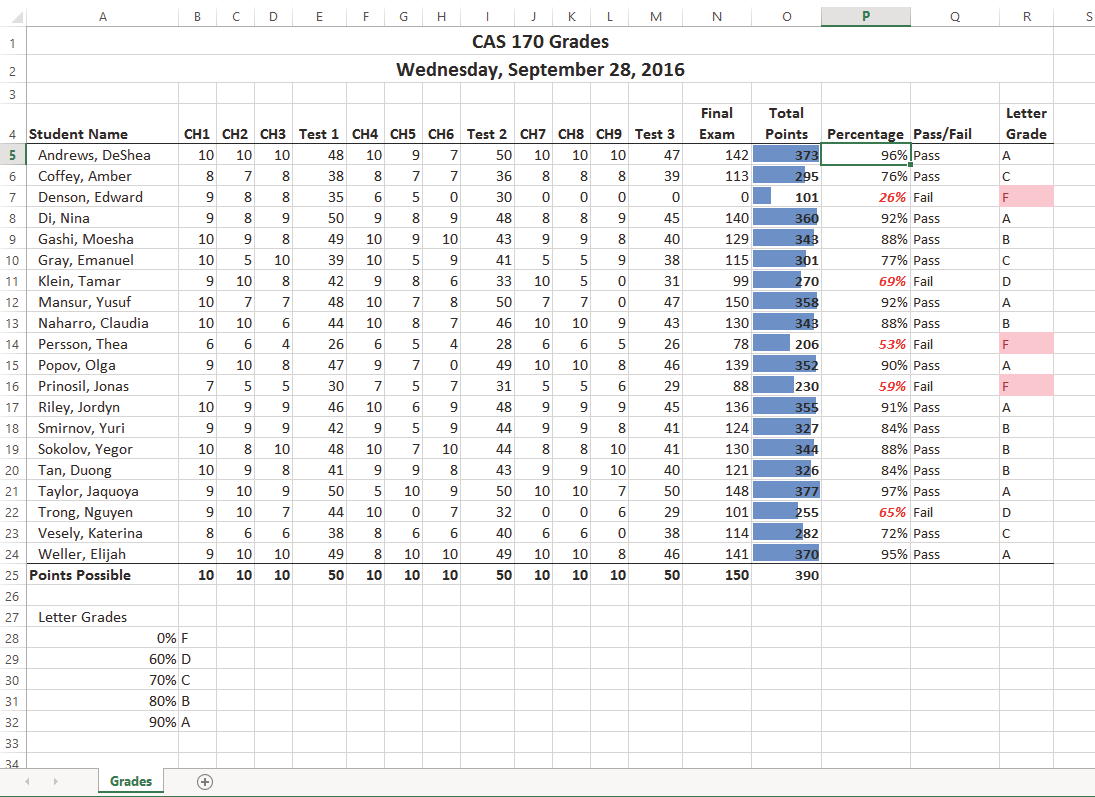
\includegraphics[width=\maxwidth{.95\linewidth}]{gfx/ch03_fig25}
	\caption{Completed Ch3 Gradebook}
	\label{03:fig25}
\end{figure}


\subsection{Setting the Print Area}

Before you consider this workbook finished, you need to prepare it for printing. The first thing you
will do is set the Print Area so that the table of Letter Grades in A27:B32 does not print.

1. Select A1:R25. This is the only part of the worksheet that you want to have print.
2. On the Page Layout ribbon, click the Print Area button. Choose Set Print Area from the menu.

Next you will preview the worksheet in Print Preview to check that the print area setting worked, as
well as make sure it is printing on one page.

1.   View the workbook in Print Preview.
2.   Set the page orientation to Landscape.
3.   Change the page scaling if needed so that the entire worksheet prints on one page.
4.   Save and close the CH3 Gradebook workbook.
5.   Compare your work with the self-check answer key (found in the Course Files link) and then
submit the CH3 Gradebook workbook as directed by your instructor.









\section{Preparing to Print}

\begin{center}
	\begin{objbox}{Learning Objectives}
		\begin{itemize}
			\setlength{\itemsep}{0pt}
			\setlength{\parskip}{0pt}
			\setlength{\parsep}{0pt}

			\item Locate and fix formatting consistency errors.
			\item Apply new formatting techniques.
			\item Use Print Titles to repeat rows and columns on each page of a multiple page worksheet.
			\item Control where page breaks occur in a multiple page worksheet.
			
		\end{itemize}
	\end{objbox}
\end{center}



In this section, we will review a worksheet for formatting consistency, as well as learn two new
formatting techniques. This worksheet currently prints on four pages, so we will learn new page setup
options to control how these pages print. A new data file will be used for this section.

\subsection{Reviewing Formatting for Consistency}

Download Data File: CH3 PTP Data

You have been given a workbook with data about the national parks in the western United States.
Your coworker formatted the workbook and has asked you to review it for consistency. You also need
to prepare it for printing. Figure 3.26 shows how the second page of the finished worksheet will
appear in Print Preview.



\begin{figure}[H]
	\centering
	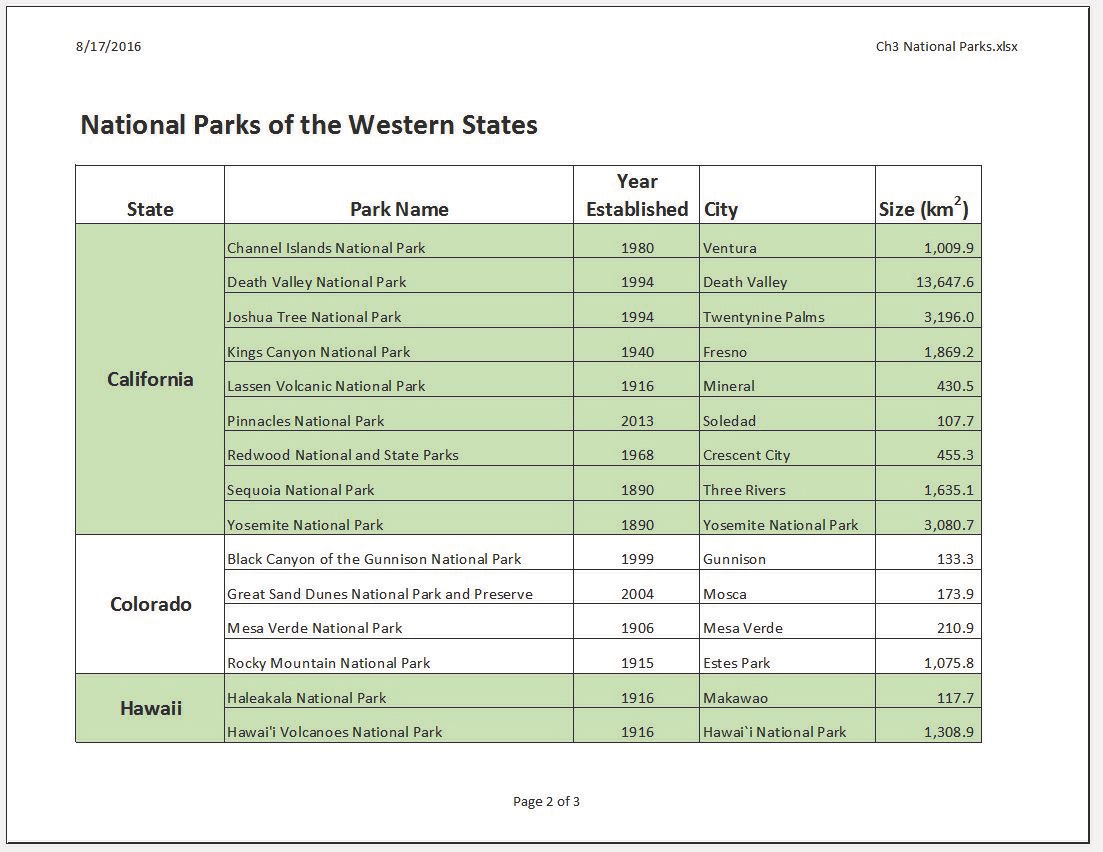
\includegraphics[width=\maxwidth{.95\linewidth}]{gfx/ch03_fig26}
	\caption{Completed National Parks worksheet}
	\label{03:fig26}
\end{figure}



\subsection{Reviewing Formatting for Inconsistencies}

The first thing you are going to do is review the worksheet for formatting inconsistencies.

1. Open the data file named CH3 PTP Data and use the File/Save As command to save it with the
new name CH3 National Parks.
2. Scroll through the worksheet and locate the following formatting errors:

* The formatting of the Utah label does not match the other states.
* The Year Established values for Hawaii are not center aligned like the other years.
* The cells for the Nevada data should have the same green fill color as the other alternating
states.
* The number of digits after the decimal place for the Size values is inconsistent. Also, these
values should be formatted with Comma style to make them easier to read.

3. To fix these errors, complete the following steps:


* Merge \& Center A34:A38. Change the font size to 16 and apply Bold format.
* Center align C28:C29.
* Apply the green fill color to A31:E31 (be sure to match the green fill color of the other states).
* Select E4:E43 and apply Comma Style. Use Increase Decimal and/or Decrease Decimal until one digit appears after the decimal place for all values.

4. While you're fixing errors, proofread the sheet and correct any typos.

\subsection{Fine-Tuning Formatting}

Now that you have fixed the inconsistencies in the formatting, you decide to apply some formatting
techniques to make the worksheet look even better. You are going to start by vertically aligning the
names of the states within the cells.

1. Select A4:A43 (the cells with the state labels).
2. Click the Home tab on the ribbon.
3. In the Alignment group, click the Middle Align button (see Figure 3.26). Notice that the names
of the states are now centered between the top and bottom borders of the cells.


\begin{figure}[H]
	\centering
	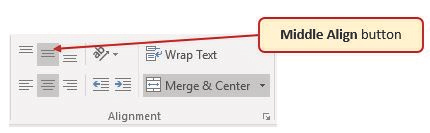
\includegraphics[width=\maxwidth{.95\linewidth}]{gfx/ch03_fig27}
	\caption{Alignment Group}
	\label{03:fig27}
\end{figure}



The next new formatting skill is to change the label in E3 from Size (km2) to Size (km2) with the 2
after km formatted with superscript.

1. Double-click on cell E3 to enter Edit mode
2. Select just the 2 (be careful not to select anything else).
3. On the ribbon (Home tab) click the dialog box launcher arrow in the Font group.
4. In the Effects section of the Format Cells dialog box, check the box for Superscript (see Figure
3-27). Click OK.
5. Save the CH3 National Parks file.




\begin{figure}[H]
	\centering
	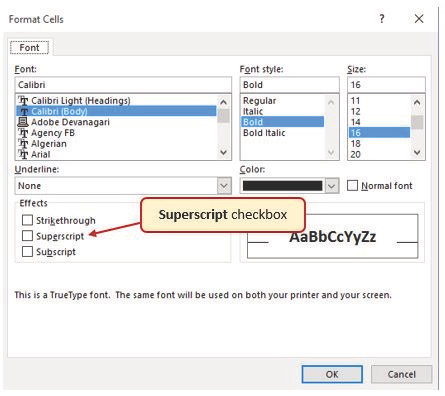
\includegraphics[width=\maxwidth{.95\linewidth}]{gfx/ch03_fig28}
	\caption{Font Tab in Format Cells Dialog Box}
	\label{03:fig28}
\end{figure}


\subsection{Repeating Column (And Row) Labels}

Now that you have fixed the cell and text formatting, you are ready to review the worksheet in Print
Preview. You will notice that the worksheet is printing on multiple pages, and you cannot tell what
each column of data represents on some of the pages.

1. With the CH3 National Parks file still open, go to Backstage View by clicking the File tab on the
ribbon. Select Print from the menu.
2. Click through each of the pages. The worksheet is currently printing on four pages, with the
City and Sizes columns printing on separate pages from the rest of the data.
3. Change the Orientation from Portrait to Landscape. This fits all of the columns on one page.All
of the columns are now on the same page, but the second and third pages have no column labels
to identify what information is in each column. You are going to use Print Titles to repeat the
first three rows of the worksheet on each of the printed pages. To set Print Titles you need to
exit Print Preview.
4. Exit Backstage View then click the Page Layout tab on the ribbon.
5. Click the Print Titles button in the Page Setup group on the ribbon. The dialog box shown
in Figure 3.28 should appear.


\begin{figure}[H]
	\centering
	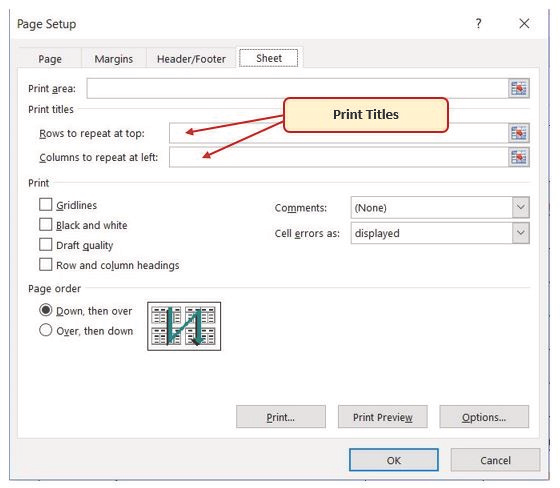
\includegraphics[width=\maxwidth{.95\linewidth}]{gfx/ch03_fig29}
	\caption{Print Titles}
	\label{03:fig29}
\end{figure}



6. Click in the Rows to repeat at top: box. Be sure your insertion point is blinking in that box before
moving on to the next step.
7. In the worksheet, select Rows 1 through 3. The text $1:$3 should now appear in the Rows to
repeat at top: box.
8. Click OK.

You will not see a change to the worksheet in Normal view, so you will need to return to Print
Preview. While looking in Print Preview, you will notice that the pages are breaking in inconvenient
places.

1. Go to Print Preview and look at each of the pages. Notice that the first three rows are now
repeated at the top of each page.
2. Exit Backstage View.

\begin{center}
	\begin{sklbox}{Skill Refresher}
		\textbf{Creating Print Titles}
		\\
		\begin{itemize}
			\setlength{\itemsep}{0pt}
			\setlength{\parskip}{0pt}
			\setlength{\parsep}{0pt}

			\item Open the Page Setup dialog box and click the Sheet tab.
			\item Click in the Rows to repeat at top: box or the Columns to repeat at left: box.
			\item Click in the worksheet and select the row(s) or column(s) that you want to repeat on each page.
						
		\end{itemize}
	\end{sklbox}
\end{center}


\subsection{Inserting Page Breaks}

Notice that the data for California is split between the first and second pages. You want all of the data
for each state to be together on the same page, so you need to control the page breaks. You are going
to start by inserting a page break before the California data to force it to start on the second page,
then you will move the page break for the third page if needed. To make these changes you are going
to work in Page Break Preview.

1. Click the View tab on the ribbon then click Page Break Preview in the Workbook Views Group.
Your screen should look similar to Figure 3.29.


\begin{figure}[H]
	\centering
	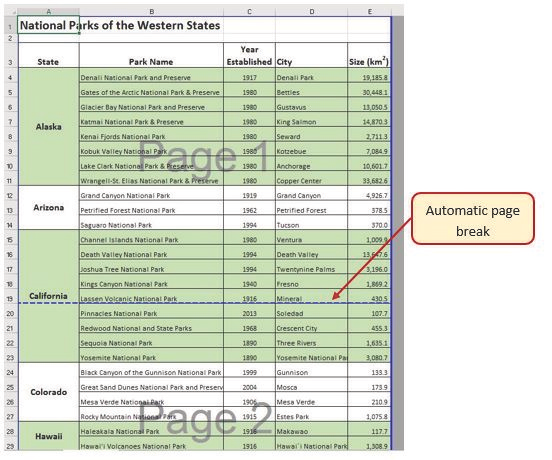
\includegraphics[width=\maxwidth{.95\linewidth}]{gfx/ch03_fig30}
	\caption{Page Break Preview}
	\label{03:fig30}
\end{figure}


In Page Break Preview, automatic page breaks are displayed as dotted blue lines. Notice the dotted
blue lines after rows 19 and 35. These lines indicate where Excel will start a new page. For this



worksheet, you want the first page to break before the California data, so you are going to insert a
manual page break.

1. Select cell A15. When inserting a page break, you select the cell below where you want the page
break to appear.
2. Click the Page Layout tab on the ribbon.
3. Click the Breaks button in the Page Setup group (see Figure 3.30).
4. Select Insert Page Break from the menu. There is now a solid blue line after row 14, which
indicates a manual page break that was inserted.
5. Go to Print Preview. Notice that the California data now starts on the second page.


\begin{figure}[H]
	\centering
	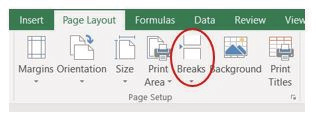
\includegraphics[width=\maxwidth{.95\linewidth}]{gfx/ch03_fig31}
	\caption{Breaks Button on Page Layout tab}
	\label{03:fig31}
\end{figure}


While looking at each page in Print Preview you decide that the third page should start with Montana.
To make this change you are going to move the automatic page break that appears after Nevada.

1. Exit Backstage View. Switch back to Page Break Preview if needed.
2. Locate the next dotted blue line (automatic page break).
3. Put your pointer over the dotted blue line and it will switch to a vertical double-headed arrow.
Click on the dotted blue line and drag it above Montana.
4. Release the mouse button when the line is above row 30 (above Montana). The line will now be a
solid blue line, indicating a manual page break.
5. Go to Print Preview. The Montana data now appears at the top of the third page.

While evaluating the pages in Print Preview you decide that there is too much white space at the
bottom of the pages. To fix this, you are going to center the contents vertically on the pages.

1. Click the Page Setup link at the bottom of the Settings section of Backstage View to open the
Page Setup dialog box.
2. Click on the Margins tab.
3. In the Center on page section, check the box for Vertically then click OK.
4. Review each page in Print Preview to see the changes. Exit Backstage View.

\subsection{Creating a Header and Footer Using Page Layout View}

Now that the worksheet is printing on three pages, with page breaks in appropriate places, you are
ready to add a header with the current date and filename. You will also add a footer with the page
number and the total number of pages that will appear as Page 1 of 3. You are going to edit the header
and footer in Page Layout View.



1. Click the View tab on the ribbon and click the Page Layout button in the Workbook Views
group.
2. The white space at the top of the worksheet should say Add header. Place the mouse pointer
over the left section of the Header and click to activate that section.
3. Click the Header \& Footer Tools Design tab on the ribbon.
4. Click the Current Date button in the Header \& Footer Elements group (see Figure 3.31).
Inserting the date this way will insert a field that will update every time the workbook is opened.
5. Click in the right section of the Header. Click the Filename button in the Header \& Footer
Elements group (see Figure 3.31). Inserting the filename this way will insert a field that will
update if the filename is changed.
6. Click the Go to Footer button in the Navigation group of commands.
7. In the center section of the footer, type the word Page with a space after it.
8. Click the Page Number button in the Header \& Footer Elements group (see Figure 3.31), then
type a space after the \&[Page] code that appears.
9. Type the word of with a space after it, then click the Number of Pages button in the Header \&
Footer Elements group (see Figure 3.31). The footer should match Figure 3.32.
10. Click anywhere on the worksheet to close the Footer editing.
11. Review the worksheet again in Print Preview. Pay careful attention to the page numbers in the
footer to ensure they will print correctly, then exit Backstage View.
12. Save the CH3 National Parks workbook.
13. Compare your work with the self-check answer key (found in the Course Files link) and then
submit the CH3 National Parks workbook as directed by your instructor.


\begin{figure}[H]
	\centering
	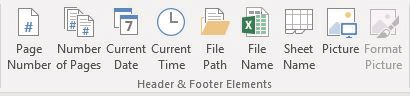
\includegraphics[width=\maxwidth{.95\linewidth}]{gfx/ch03_fig32}
	\caption{Header \& Footer Elements buttons}
	\label{03:fig32}
\end{figure}

\begin{figure}[H]
	\centering
	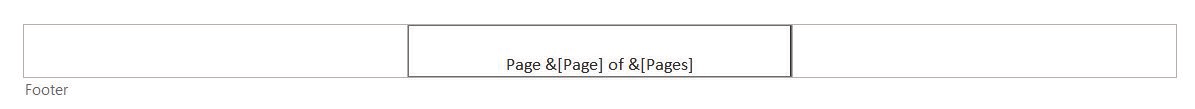
\includegraphics[width=\maxwidth{.95\linewidth}]{gfx/ch03_fig33}
	\caption{Completed Footer}
	\label{03:fig33}
\end{figure}



\begin{center}
	\begin{sklbox}{Skill Refresher}
		\textbf{Inserting Page Numbers}
		\\
		\begin{itemize}
			\setlength{\itemsep}{0pt}
			\setlength{\parskip}{0pt}
			\setlength{\parsep}{0pt}

			\item In Page Layout View, click in the section of the header or footer where you want the page number to appear.
			\item Type the word Page, followed by a space, and then click the Page Number button in the Header \& Footer Elements group on the Header \& Footer Tools Design ribbon. This will create Page 1.
			\item If desired, type a space after the \&[Page] code then type the word of followed by a space. Then click the Number of Pages button. This will create Page 1 of 4.
			
		\end{itemize}
	\end{sklbox}
\end{center}


\begin{center}
	\begin{tkwbox}{Key Take-Aways}
		\textbf{Preparing to Pring}
		\\
		\begin{itemize}
			\setlength{\itemsep}{0pt}
			\setlength{\parskip}{0pt}
			\setlength{\parsep}{0pt}

			\item Always check the formatting of your worksheets for consistency.
			\item If a worksheet is printing on multiple pages, use Print Titles to repeat rows at the top and/or columns at the left of every page to make it easier to interpret the data.
			\item Insert manual page breaks as needed in Page Break Preview to control where a new page begins.
			\item Multiple page worksheets should include the page number in either the header or footer. Be sure to insert the Page Number element so that the correct page number will display on each page of the worksheet.
			
		\end{itemize}
	\end{tkwbox}
\end{center}


\section{Chapter Practice}




\subsection{Household Budget}

Download Data File: PR3 Data

Elijah and Kelly Williams are a recently married couple living in Portland, Oregon. Elijah works part
time and attends the local community college. Kelly works as a marketing manager at a clothing
company in North Portland. They are trying to decide if they can afford to move to a better
apartment, one that is closer to work and school. They want to use Excel to examine their household
budget. They have started their budget spreadsheet, but they need your help with it.

1. Open the file named PR3 Data and then save it as PR3 Williams.
2. Insert two new rows at the top of the worksheet.
3. Enter the following text:

A2        Category
B2        Item
C2        January
O2        Yearly Total (adjust column width as needed to fit this text)

1. Using the text in cell C2, use Autofill to fill in the months February through December in cells
D2:N2. Adjust column widths as needed to fit the names of the months in these columns.
2. Bold and center align all of the headings in Row 2.
3. Type “Williams Family Budget” in A1. Merge \& Center A1:O1. Make this text 22 point bold.
4. Next you need to complete the monthly values for some of the income and expense items. In the
rows for Income \#1, Income \#2, Mortgage/Rent, Homeowners/Rent Insurance, Car Insurance,
Car Payment, and Gym Fees/Memberships, copy the values for January to the cells for February
through December.
5. Use the Totals tab in the Quick Analysis tool to add the SUM to Column O. Delete the formulas
from O7, O17, O24, O32, and O38.
6. In C6: O6, use the SUM function to calculate the Total Income for each month.
7. Similar to step 6, use the SUM function to calculate the Total Home Expenses, Total Daily
Living Expenses, Total Transportation Expenses, Total Entertainment Expenses, and Total
Personal Expenses for each month.
8. Use the SUM function to calculate the Yearly Total Personal Expenses in cell O45.
9. Format the numerical data in Row 3 as Currency with no decimal places. Format all the total
rows as Currency with no decimal places and with a top border.


10. Apply the Comma format with no decimal places in all the other rows.
11. In A47, type “Total Expenses”.
12. In C47, enter a formula that adds together all of the expense category totals for January. Copy
the formula in C47 to D47:O47.
13. In A49, type “NET INCOME”. Bold and indent this text.
14. In C49, enter a formula that calculates the difference between Total Income and Total Expenses
(=Total Income-Total Expenses) for January. Copy this formula to D49:O49.
15. Format the data in Rows 47 and 49 as Currency with no decimal places. Bold O47 and O49. Add
a Top and Double Bottom Border to the data in Row 49.
16. Select C49:N49. Use the Quick Analysis tool to add data bars to this data.
17. In B50, type “New Apartment?”. Enter an IF statement in C50 that displays the word “No” if the
amount in C49 is less than or equal to zero and “Maybe” if the amount is greater than zero.
Copy C50 to D50:N50.
18. Check to see if your IF statement worked correctly in row 50. If the cells say “No” when the data
bar in the cell above it is red and “Maybe” when the data bar in the cell above it is blue, your IF
statement is correct.
19. Review the worksheet in Print Preview. Make any changes needed to make the worksheet print
on one page with landscape orientation.
20. Save the PR3 Williams workbook.
21. Compare your work with the self-check answer key and then submit the PR3 Williams
workbook as directed by your instructor.




\section{Chapter Scored}




\subsection{Astrocoffee Company}

Download Data File: SC3 Data

AstroCoffee: Cynthia McHenry owns a coffee supply company named AstroCoffee. She needs some
help writing the formulas for the order form she uses to invoice customers. You will need to write the
formulas for all of the calculations on the form. Some of the more complex parts are determining if
the customer will get a discount (based on the customer status) as well as the shipping charge (orders
over \$200 get free shipping). You will use IF functions for both of those calculations.

1. Open the SC3 Data workbook and save the workbook as SC3 AstroCoffee.
2. Enter the following order information:
Order \#: 45676
Order Date: use a function that displays the current date
3. Enter the following Billing Information:
Edwina Copeland
4270 Heron Way Portland, OR 97225
503-779-1873
edwina.copeland@hmail.com
4. For the Shipping Information, create formulas using cell references to display the corresponding
information from the Billing Information section. For example, the Customer cell will display
the name of the customer in cell C11.
5. In the range B19:E22, enter the following item orders:

Item \# Description                       Qty Unit Price
K56    Dark Mocha K-Cups (12 pack)       1    10.99
G03    Decaf Dark Roast – Ground (1 lb.) 3    12.99
B07    Dark Roast – Whole Bean (1 lb.)   2    13.99
K52    Chai Latte K-Cups (12 pack)       3    12.99

6. In cell F19, enter an IF function that tests whether the order quantity in cell D19 is greater than
0 (zero). lf it is, return the value of the Qty (in D19) multiplied by the Unit Price (in E19);
otherwise, return no text by entering “”.
7. Copy/fill this formula into the other cells in the range F19:F25. Hint: be sure to copy the formula to
all of the Item Total cells, even if it is a blank row. You want the worksheet to be prepared for orders with
more items in the future.


8. In cell F26, calculate the sum of all of the Item Total cells.
9. In cell F27, use an IF function to calculate the discount amount for this order based on the
customer’s status (which is found in F16). If the customer’s status is Preferred, the discount
amount will be the Order Subtotal times the discount percentage found in cell B29; otherwise
the discount amount will be 0 (zero). Hint: You will need to use a formula for the Value if True
argument.
10. Calculate the Discounted Total for this order in cell F28. Hint: Use a simple subtraction formula.
11. In cell F29, use an IF function to display the correct Shipping Charge, based on the amount of
the Discounted Total. If the Discounted Total is greater than or equal to the Free Shipping
Minimum found in cell B28, the Shipping Charge is 0 (zero); otherwise, the Shipping Charge is
5\% of the Discounted Total. Hint: You will need to use a formula for the Value if False to calculate what
5\% of the Discounted Total will be.
12. Calculate the Invoice Total in cell F31. Hint: This will be the total of the Discounted Total and the
Shipping Charge.
13. Review the worksheet in Print Preview. Make any changes needed to make the worksheet print
on one page.
14. Save the SC3 AstroCoffee workbook.
15. Submit the SC3 Astro Coffee workbook as directed by your instructor.





